\chapter{Classificação de padrões arquiteturais organizacionais para SMA}\label{sec:criterios_categoria}

\citeonline{malone1990organizing}, \citeonline{sycara1998multiagent}, \citeonline{Argente200655} abordam, em seus trabalhos, estruturas de coordenação de SMA a partir do emprego da Teoria Organizacional. Após a análise das categorias de cada trabalho, observou-se que as mesmas possuíam o mesmo conceito, diferenciando-se apenas pelo nome e pelos autores dos trabalhos que as citam. São, portanto, equivalentes e sinônimos para este trabalho: \textit{Market} e \textit{Organic}; \textit{Hierarchy} e \textit{Mecanic}. 

A seguir, tais categorias serão apresentadas em detalhe e fomentaram as categorias e subcategorias, as quais os padrões definidos no catálogo foram classificadas. A Figura \ref{fig:my_patterns} ilustra a estrutura das categorias e subcategorias. 

\begin{figure}[H]
    \centering
    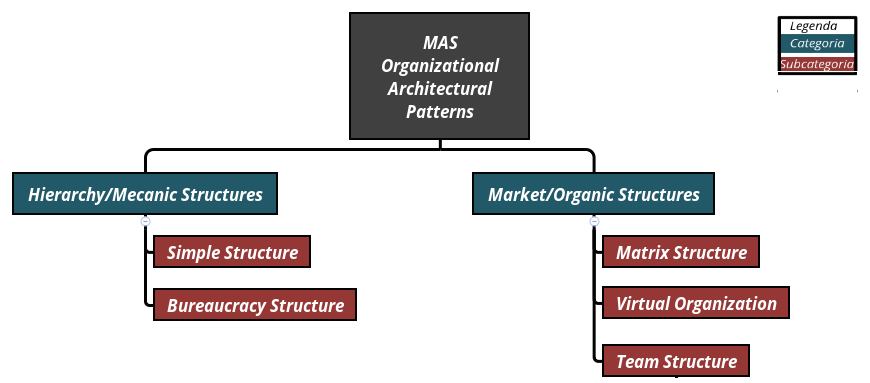
\includegraphics[scale=0.5]{figuras/MAS_Categories.png}
    \caption{Categorias e Subcategorias. Fonte: Autora.}
    \label{fig:categories}
\end{figure}

\section{Categorias \textit{Mecanic} e \textit{Organic}}

\citeonline{Argente200655} realizam uma revisão das organizações humanas mais conhecidas para que possam ser aplicadas no campo de SMAs. Tais organizações podem ser usadas como base para descrever papéis, padrões e conexões que colaboram com a definição de arquiteturas para SMAs. A Teoria Organizacional (\textit{Organizational Theory}) analisa como funcionam as organizações, suas características principais, as características mais relevantes de seus membros, seus papéis, as relações dos membros, a cadeia de comando, as regras e normas que regem a organização, dentre outros aspectos. 

Nesse sentido, \citeonline{Argente200655} definem dois tipos de organizações humanas: mecânicas e orgânicas. Nas organizações mecânicas, as tarefas são definidas com precisão, e são divididas em partes separadas e especializadas. Existe uma hierarquia de autoridade rígida. Os processos de conhecimento e raciocínio também são centralizados no topo da hierarquia. As comunicações são, principalmente, verticais (entre supervisores e subordinados). São três exemplos deste tipo de organização: \textit{Simple Structure}, \textit{Bureaucracy Structure} e \textit{Matrix Structure}. A Figura \ref{fig:organizational_feature} apresenta características de cada uma dessas organizações humanas.


\begin{figure}[H]
    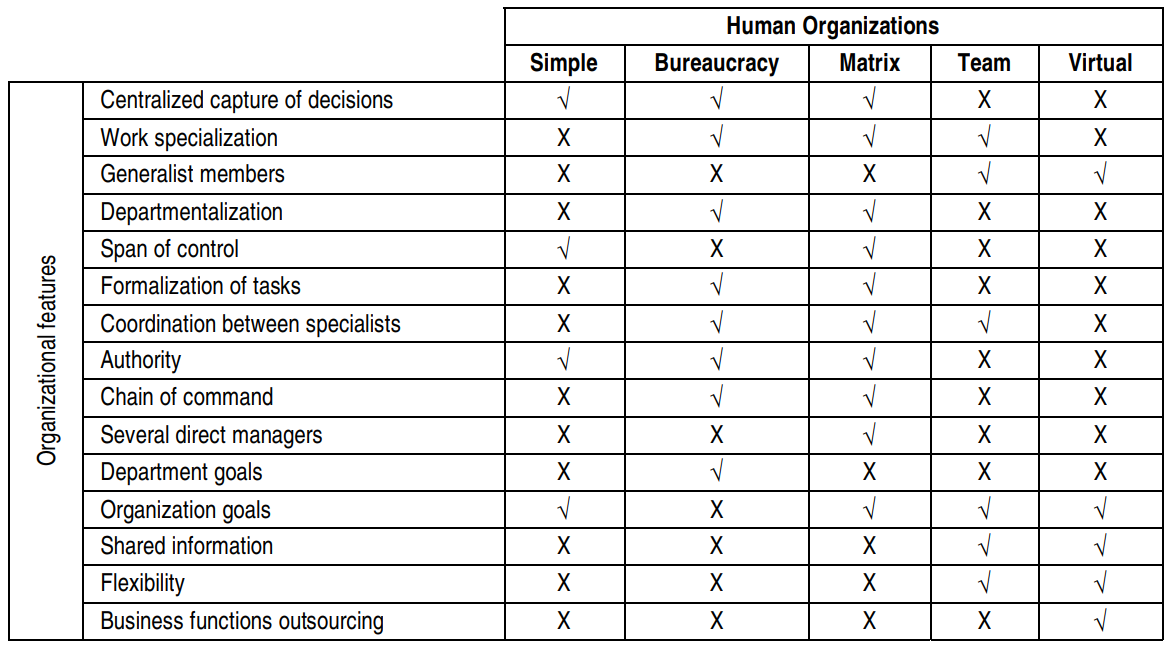
\includegraphics[scale=0.35]{figuras/organizational_features.png}
    \centering
    \caption{Características de organizações humanas. Fonte: \citeonline{Argente200655}.}
    \label{fig:organizational_feature}
\end{figure}

Nas organizações orgânicas, as tarefas são ajustadas e redefinidas por meio de trabalho colaborativo em grupos \cite{Argente200655}. Existem menos níveis de autoridade e controle, de modo que o controle do conhecimento e das tarefas são distribuídos. Todos os membros devem contribuir para a tarefa comum do departamento. As comunicações são principalmente horizontais entre membros do mesmo departamento, ou mesmo entre diferentes departamentos. Desta forma, eles podem oferecer respostas rápidas e flexíveis. São exemplos deste tipo de organização: \textit{Team Structure} e \textit{Virtual Organizations}.

A subcategoria \textbf{\textit{Simple Structure}} representa uma organização com poucos departamentos, onde um indivíduo centraliza a captura de decisões \cite{Argente200655}. Esta estrutura apresenta um alto grau de controle, pois o gerente dirige um grande número de pessoal. Este tipo de organização é, frequentemente, empregado em pequenas empresas, onde o gerente e proprietário são a mesma pessoa, bem como em grandes empresas quando o controle é centralizado em um indivíduo. 

Esta organização é simples: as responsabilidades são claras, as comunicações são diretas e a captura de decisões e sua execução é rápida. No entanto, é recomendada somente para organizações pequenas, pois há pouca formalização e o gerente deve lidar com muitas informações. Já que tudo depende de uma única pessoa, se essa pessoa falhar ou tomar uma decisão errada, a empresa pode ser prejudicada \cite{Argente200655}.

A subcategoria \textit{\textbf{Bureaucracy Structure}} é caracterizada, principalmente, por tarefas operacionais e de rotina com alta especialização. Há também muitas regras e regulamentos formalizados. Por haver diversos departamentos, é ocasionado um baixo nível de controle, com o qual os gerentes controlam um pequeno grupo de pessoas ou departamentos \cite{Argente200655}. %; portanto, muitos níveis de gerenciamento podem ser estabelecidos (dependendo do tamanho total da empresa).

Há uma autoridade central e a tomada de decisões segue uma cadeia de comando. Entre suas vantagens, esta estrutura permite que as atividades padrão sejam realizadas de forma muito eficaz. Os especialistas são reunidos nos mesmos departamentos, facilitando as comunicações entre os funcionários. Graças à ampla presença de regras e regulamentos e à padronização das operações, a tomada de decisões é centralizada em gerentes executivos \cite{Argente200655}.

No entanto, a alta especialização das tarefas pode criar conflitos em unidades ou departamentos. Os gerentes podem estar mais focados em alcançar seus objetivos individuais do que os objetivos gerais da organização \cite{Argente200655}.

Além disso, os gerentes podem estar excessivamente concentrados em seguir as regras, o que dificulta suas decisões quando confrontados com novas situações. Portanto, esses tipos de organizações tem dificuldades em responder às mudanças externas \cite{Argente200655}.

A subcategoria \textbf{\textit{Matrix Structure}} possui dois supervisores: o gerente do departamento funcional e o gerente do produto. Portanto, existem duas cadeias de controle. Esse tipo de estrutura é muito comum em empresas de engenharia e gerenciamento de projetos.
Facilita a coordenação entre funcionários quando há numerosas atividades complexas e interdependentes \cite{Argente200655}.

Outra vantagem consiste na melhoria das comunicações e ampliação da flexibilidade. Também reduz a possibilidade dos membros se concentrarem nos objetivos individuais de seus departamentos mais do que nos objetivos gerais da organização. Da mesma forma, facilita a localização efetiva de especialistas \cite{Argente200655}.

No entanto, pode haver confusão na tomada de decisões, pois existem duas cadeias de comando. Além disso, esta estrutura promove lutas de poder e pode criar tensão, que pode ser diminuída usando técnicas burocráticas, como, por exemplo, uma formalização maior das regras \cite{Argente200655}.

A subcategoria \textit{\textbf{Team Structure}} elimina barreiras departamentais e descentraliza a tomada de decisão. Equipes ou grupos representam um sistema com vários atores que possuem um objetivo comum: a realização da tarefa global do sistema \cite{Argente200655}.

Esta tarefa é dividida em sub-tarefas, que são atribuídas aos membros mais qualificados do grupo. Além disso, os membros compartilham todas as informações e estão em constante comunicação uns com os outros. A coordenação entre atores é obtida usando decisões e planos mutuamente aceitos \cite{Argente200655}. 


A subcategoria \textit{\textbf{Virtual Organization}} consiste em uma empresa que terceiriza suas principais funções comerciais. Várias redes de contato são criadas, o que permite que a empresa contrate funções comerciais que os gerentes acreditam que possam ser feitas por outras empresas de uma maneira melhor ou a um custo menor. Esta estrutura oferece flexibilidade, mas reduz o controle de gerenciamento em partes fundamentais da organização \cite{Argente200655}. 

\section{Categorias \textit{Markets} e \textit{Hierarchies}}
%Nesta Seção são conceituadas as categorias de estruturas organizacionais para SMA a partir da qual possibilita a elaboração dos critérios para sua classificação (Seção \ref{sec:criterios_categoria})

%\subsubsection{Categorias de estruturas organizacionais para SMA}

\citeonline[pág. 61]{malone1990organizing} considera três processos fundamentais de coordenação de SMA:

\begin{description}
    \item[• Ajuste mútuo:] trata-se do modo mais simples de coordenação, no qual dois ou mais agentes compartilham seus recursos visando atingir um objetivo comum. Nenhum agente tem controle prévio sobre os outros, e a tomada de decisões é um processo conjunto;
    \item[• Supervisão direta:] ocorre quando dois ou mais agentes já estabeleceram um relacionamento em que um agente tem algum controle sobre os outros. Nesta forma de coordenação, o supervisor controla o uso de recursos compartilhados - como trabalho humano, tempo e dinheiro do processo de computador - pelos subordinados, e também pode prescrever certos aspectos de seus comportamentos, e
    \item[• Padronização:] ocorre quando o supervisor estabelece procedimentos padrão para subordinados a serem seguidos em várias situações. Os procedimentos de rotina em empresas ou em software são exemplos de coordenação por meio da padronização.
\end{description}

Por meio desses processos fundamentais de coordenação podem ser elaborados sistemas de coordenação mais sofisticados \cite[pág. 63]{malone1990organizing}. São eles:

\begin{description}
    \item[• \textit{Markets}/Mercados:] podem ser considerados uma forma de organização baseada em ajuste mútuo. Os agentes, cada um dos quais controla recursos escassos - como, por exemplo, trabalho, matéria-prima, bens e dinheiro, concordam em compartilhar alguns de seus respectivos recursos para alcançar o objetivo mútuo. Os recursos são trocados, com ou sem custos explícitos. Uma vez que um contrato foi feito, existe um acordo em que o ``comprador"  se torna o supervisor do fornecedor, e
    \item[• \textit{Hierarchies}/Hierarquias:] baseiam-se em processos de supervisão direta. Um grande grupo pode ser dividido em subgrupos se a maior parte da transferência de informações necessária pode ocorrer em subgrupos e se as poucas interações entre subgrupos podem ser tratadas por supervisores. Nesse caso, pode-se utilizar como estratégia a hierarquia. Os subgrupos podem ser coordenados por ajuste mútuo ou por controle hierárquico, dependendo do domínio do aplicativo e das características da tarefa.
\end{description}

\citeonline{sycara1998multiagent}, de modo semelhante, apresenta \textit{Market} e \textit{Hierarchy} como exemplo de organizações que são exploradas na literatura. Complementando o conceito de \textit{Hierarchies}, \citeonline{sycara1998multiagent} define que esta estrutura é formada por uma autoridade para tomada de decisão e controle concentrada em um único solucionador de problemas (ou grupo especializado) em cada nível da hierarquia. A interação é através da comunicação vertical do agente superior ao subordinado e vice-versa; de modo que agentes superiores exerçam controle sobre recursos e tomada de decisões.

Na estrutura \textit{Market}, o controle é distribuído aos agentes que competem por tarefas ou recursos através de lances e mecanismos que envolvem contratos. Os agentes interagem através de uma variável, como o custo, que é usado para avaliar os serviços \cite{sycara1998multiagent}.

\section{Critérios para classificação em categorias e subcategorias}

Baseando-se nos conceitos abordados até o momento, foram elencados critérios para classificar as estruturas organizacionais dos padrões arquiteturais identificados para que sejam catalogados. Os critérios para classificar uma estrutura organizacional como \textit{Hierarchy/Mecanic} são:

\begin{itemize}
    \item Há uma autoridade - ou seja, um agente ou um grupo de agentes superior - para a tomada de decisão e o controle de recursos;
    \item A comunicação dá-se verticalmente; da autoridade para o subordinado e vice-versa, e
    \item A autoridade pode prescrever aspectos do comportamento dos subordinados.
\end{itemize}

Os critérios para classificar uma estrutura organizacional como \textit{Markets/Organic} são:

\begin{itemize}
    \item Nenhum agente possui controle sobre os demais;
    \item Dois ou mais agentes compartilham seus recursos visando atingir um objetivo comum;
    \item Os agentes competem por tarefas ou recursos através de lances ou contratos, e
    \item A tomada de decisões ocorre mutuamente.
\end{itemize}

\section{Elementos para a descrição dos padrões arquiteturais}\label{subsec:elementos_descricao_dos_padroes}

Os elementos fundamentais para descrever os padrões arquiteturais identificados neste catálogo são:

\begin{description}
    \item[Nome do padrão:] nome do padrão encontrado na literatura;
    \item[Referências:] referências para os trabalhos que descrevem o padrão;
    \item[Categoria:] classificação do padrão em \textit{Market} - e subcategorias \textit{Simple Structure} e \textit{Bureaucracy Structure} -, e \textit{Hierarchy} - com subcategorias \textit{Matrix Structure}, \textit{Virtual Organization} e \textit{Team Structure};
    \item[Problema:] problema em que o padrão busca solucionar, descrevendo-se seus objetivos;
    \item[Solução:] instruções descrevendo como o problema pode ser resolvido;
    \item[Protocolos associados:] este elemento é opcional. Caso o padrão esteja implementado em alguma plataforma acessível, os protocolos ou bibliotecas associados serão referenciados;
    \item[Modelagem:] diagramas disponibilizados pela literatura representando o padrão. A notação utilizada deve ser apropriada para SMA como, por exemplo, diagrama de sequência UML \cite{larman2002utilizando};
    \item[Exemplo:] quando disponível na literatura, será apresentado um exemplo prático do padrão arquitetural, podendo conter trechos de código e figuras que torne o exemplo mais didático, e
    \item[Implementação:] a descrição do padrão poderá conter mais um elemento: sua implementação. A implementação dependerá da viabilidade tecnológica para que seja cumprido e preenchido para cada padrão.
\end{description}


